\phantomsection


% Is it possible to keep my translation together with original text?
% https://tex.stackexchange.com/questions/5076/is-it-possible-to-keep-my-translation-together-with-original-text
\chapter[\lang{Basic concepts and Related works}{Conceitos básicos e Trabalhos relacionados}]
{
    \lang
    {Basic concepts and Related works}
    {Conceitos básicos e Trabalhos relacionados}
}
\label{sec:related}

\begin{flushright}
    \englishword{ }
\end{flushright}


% Multiple-language document - babel - selectlanguage vs begin/end{otherlanguage}
% https://tex.stackexchange.com/questions/36526/multiple-language-document-babel-selectlanguage-vs-begin-endotherlanguage
In this chapter we present the basic concepts related to trajectories in Section \ref{sec:basic_concepts}. In Section \ref{sec:related_measures} we present a review on trajectory similarity measures, where the section \ref{sec:related_raw} presents measures for raw trajectory similarity and the section \ref{sec:related_semantic} presents measures for semantic trajectory similarity.

\section{Basic concepts} \label{sec:basic_concepts}
\hl{There are three important concepts that need to be explained and defined: raw trajectory, semantic trajectory and similarity measure.}

A raw trajectory is a discrete representation of the movement of an object that can be defined as a time-ordered finite sequence of space-time points, as formalized in Definition \ref{def:raw_trajectory}. 

\begin{definition}[Raw Trajectory] \label{def:raw_trajectory}
A raw trajectory is a time-ordered sequence of points in the form R = $<p_1,...,p_n>$ where point p\textsubscript{k} $\in$ R is a tuple p\textsubscript{k} = ($x,y,t$), where $x,y$ represent the spatial location of the moving object at a time instant $t$.
\end{definition}

Figure \ref{fig:related_trajes} illustrates a example of raw trajectory $R$. The spatial coordinates are annotated next to the trajectory points and we consider the time instants as the index associated to each point. For instance, the first point of trajectory is located at the coordinates $(6,39)$ at time instant $1$.

\begin{figure}[h]
\centering
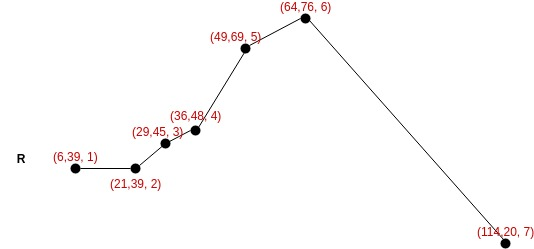
\includegraphics[width=0.65\textwidth]{Related_Works/Single_trajectory.jpg}
\caption{\label{fig:related_trajes}A raw trajectory $R$}
\end{figure}

Traditionally a trajectory is represented as stated in Definition \ref{def:raw_trajectory}, i.e., a time-ordered sequence of spatial points. Alvares \cite{alvares2007model} and Spaccapietra \cite{Spaccapietra:2008:CVT:1347466.1347785} proposed a new representation for trajectories, defining a trajectory as a time-ordered sequence of \emph{stops} and \emph{moves}, where the \emph{stops} are the most relevant parts of the trajectory.
In this work, we formally define semantic trajectory, considering its sequence of stops and moves, which is an enriched extension of the definition presented in \cite{Spaccapietra:2008:CVT:1347466.1347785}:

\begin{definition}[Semantic Trajectory]
\label{def:semantic_trajectory}
A semantic trajectory  \break
$P=\langle s_1, m_1, s_2, m_2, s_3,m_3, ...., s_k, m_k, s_{k+1} \rangle$ is a time ordered sequence of stops and moves, where each stop $s_i$ has a set of attributes $\{d_{a1}, d_{a2}, ...d_{aq}\}$ characterizing it according to q-dimensions, and each move $m_j$  has a set of attributes $\{d_{b1}, d_{b2}, ...d_{br}\}$ characterizing it according to r-dimensions. 
\end{definition}

Figure \ref{fig:related_semantic_trajes} shows a semantic trajectory $P$ representing an 1 day movement of a professor. A semantic trajectory can be enriched with the name of the place where the \emph{stop} occurred, the category of the place or the time interval that the \emph{stop} happened. The \emph{move} can be enriched with the street where the object drives, the traveled distance between two \emph{stops} or the mean velocity during \emph{move}.

\begin{figure}[h]
\centering
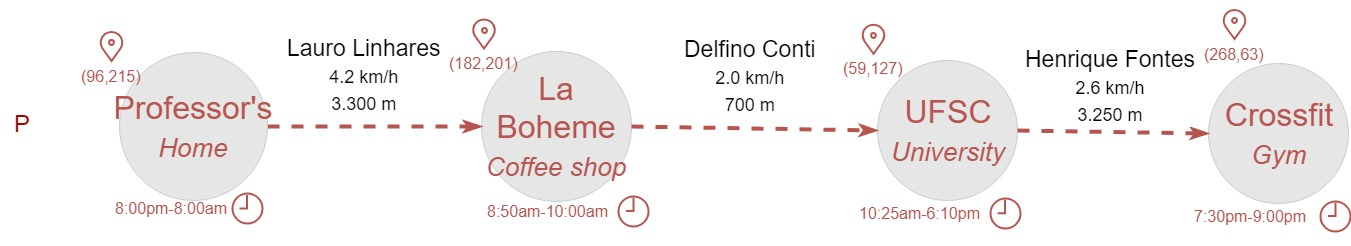
\includegraphics[width=0.85\textwidth]{Related_Works/Single_Semantic_trajectorie.jpg}
\caption{\label{fig:related_semantic_trajes}A semantic trajectory $P$ representing 1 day movement of a professor}
\end{figure}

\hl{To compare and measure two distinct trajectories we use a similarity measure. In this thesis we use the intuitive concept of similarity stated in }\cite{lin1998information}\hl{, where two objects $A$ and $B$ are said as more similar when they share more commonality between each other and they are less similar as more differences they have. We formalize the similarity measure concept according Definition }\ref{def:similarity_measure}:

\begin{definition}[Similarity Measure]
\label{def:similarity_measure}
A similarity measure on a object set $G$ is a function $sim: G \times G \to [0,1]$, such that two objects $A$ and $B$ they are more similar then the score returned by $sim(A, B)$ increases.
\end{definition}

\section{Related Trajectory Similarity Measures} \label{sec:related_measures}

Similarity measures have been proposed for several data processing and analysis techniques, such as outlier detection, top-K similarity queries, clustering, and others. In the context of trajectory data, several similarity measures were proposed for both raw trajectory data and semantic trajectory data. In this section, we present a literature review on similarity measures of raw and semantic trajectories.
The Section \ref{sec:related_raw} presents similarity measures for raw trajectories and Section \ref{sec:related_semantic} presents similarity measures for semantic trajectories.


\subsection{Related works on raw trajectory similarity measures} \label{sec:related_raw}
{As presented in Section {\ref{sec:basic_concepts},} a raw trajectory is a time-ordered sequence of points containing a spatial coordinate and a timestamp. For this reason, existing measures developed for generic time-ordered sequences or time-series can be applied to raw trajectories, even though they were not originally proposed for this purpose. At the beginning of this section, we present a distance measure proposed for time-series }\cite{berndt1994using}{ that can be adapted to work with raw trajectory data }\cite{ten2007multi}{. Then we present similarity measures developed for raw trajectories which were adapted of more general similarity measures }\cite{eiter1994computing, Ding:2008:ESJ:1440463.1440989, vlachos2002discovering, Chen:2004:MLE:1316689.1316758, Chen:2005:RFS:1066157.1066213}{ and after, a similarity measure proposed exclusively for raw trajectories }\cite{Furtado-UMS-2018}.

Throughout this section, we use a set of symbols to denote hypothetical trajectories. Table \ref{tab:symbols} summarizes the symbols used in this section.

\begin{table}[!h]
    \centering
    \resizebox{\linewidth}{!}{%
        \begin{tabular}{c|c}
             Symbol & Meaning  \\
             \hline
             $P$, $Q$ and $R$ & Trajectories \\
             $m$ and $n$ & Number of points of trajectories $P$ and $Q$, respectively \\
             $d_i$ & \emph{i}th-dimension of data in a point \\
             $w$ & Size of the window \\
             $k$ & Number of \emph{moves} in a semantic trajectory \\
             $\epsilon$ & Threshold distance between two points that match \\
             $x,y$ & Spatial coordinates \\
             $dist()$ & Distance function
        \end{tabular}
    }
    \caption{Symbol meanings}
    \label{tab:symbols}
\end{table}

An early proposed distance measure is \emph{Dynamic Time Warping} (DTW) \cite{berndt1994using}, developed for time-series. DTW is used to find the best match between the points of two time-series independent of their sizes. It creates a matrix with all possible pairs of points of the time-series with the pairwise distances as the entries.
The total distance between two trajectories is given by the sum of the entries of the minimum contiguous path in the matrix{, where the minimum contiguous path is the best alignment between two sequences of points, with the lower sum of distances of their points}. Because DTW sums the distances between all points, it is sensitive to noise. For example, when a time-series $P$ has a point that is significantly distant from all points of the time-series $Q$, even if all the other points of $P$ and $Q$ are close, their distance will be dominated by the distant point. A recursive formalization of DTW is presented in Equation \ref{func:DTW}.

\begin{equation}
\label{func:DTW}
  DTW(P, Q) = 
    \begin{cases} 
        0 & \text{if } m = n = 0\\ 
      \infty & \text{if } m = 0 \text{ or } n = 0\\ 
      dist(p_1, q_1) + min( & otherwise\\
      DTW(<p_2...p_m>,<q_2...q_n>),\\
      DTW(<p_2...p_m>, Q), \\
      DTW(P, <q_2...q_n>)) &
    \end{cases}
\end{equation}

The \emph{Multidimensional DTW} (MD-DTW) \cite{ten2007multi} extends DTW for dealing with trajectories whose points have more than one dimension. MD-DTW normalizes the distance in the different dimensions and then creates a matrix with entries as the sum of the distances in all dimensions. Finally, it runs DTW over the matrix and finds the minimum contiguous path. Figure \ref{fig:related_trajes_wDF_DTW} (left) illustrates the computation of MD-DTW between trajectories $P$ and $Q$. Its distance is calculated as the sum of the minimum contiguous path between points of $P$ and $Q$, i.e. the sum of all dashed lines, resulting in a distance of MD-DTW$(P, Q) \approx 123$.

{\emph{Discrete Fr{\'e}chet Distance} }\cite{eiter1994computing}{adapts the classical Fr{\'e}chet Distance }\cite{Frechet1906}{ to work with trajectories. This distance is popularly exemplified as \textit{the man walking dog} distance, where the two trajectories represent a dog and his owner and the Fr{\'e}chet Distance between them is the maximum size of the leash that could keep them together.}

Ding in \cite{Ding:2008:ESJ:1440463.1440989} proposes \emph{w-constrained discrete Fr{\'e}chet Distance} (wDF), which extends the Discrete Fr{\'e}chet distance \cite{eiter1994computing} by adding a temporal window, in order to consider only the pairs of points that are within a given \emph{w} time window. {As DTW, wDF calculates the distance between the trajectory points by a continuous distance function (e.g. Euclidean distance), making it sensitive to noise}. Indeed, this measure makes the assumption that the two trajectories have the same number of points, making point interpolation when necessary. The wDF distance is given by the minimum distance of all possible time windows over two trajectories, where the distance of each window is the maximum distance between all pairs of points of $P$ and $Q$ inside the window, as shown in Equation \ref{func:match_wDF}.

\begin{equation}
\label{func:match_wDF}
  wDF(P, Q) = min(\forall_{i,j=0}max(dist(P_i, Q_j))) \Rightarrow i \leq j + w \land
  j \leq P_{m} - w
\end{equation}

Figure \ref{fig:related_trajes_wDF_DTW} (right) shows trajectories $P$ and $Q$ and a \emph{w} time-window. The wDF distance between the trajectories is computed as the maximal distance found among all \emph{w}-constrained time-windows. As the time-window shifts over trajectories, the maximal distance between their points is computed, using the Euclidean distance. In the example of Figure \ref{fig:related_trajes_wDF_DTW} (right), the wDF distance is $wDF($P$, $Q$) = euclidean((6,39), (4,9)) \approx 30$.

\begin{figure}[h]
\centering
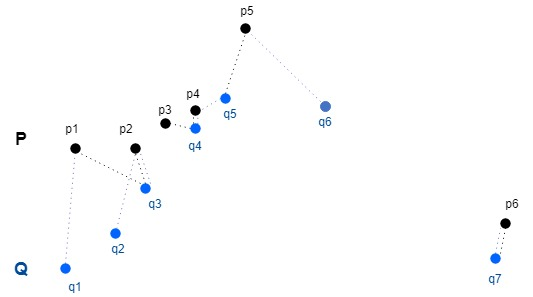
\includegraphics[width=0.45\textwidth]{Related_Works/related_trajes-DTW.jpg}
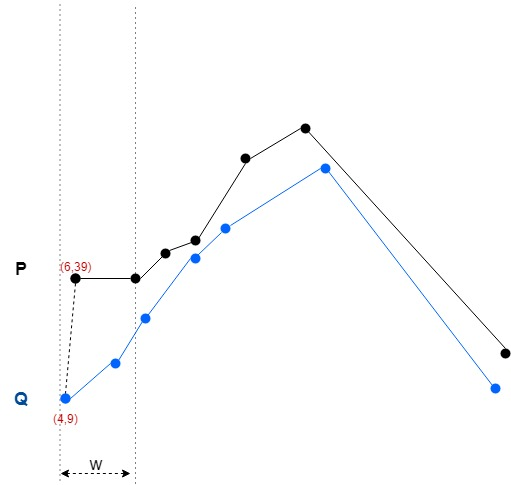
\includegraphics[width=0.45\textwidth]{Related_Works/related_trajes-wDF.jpg}
\caption{\label{fig:related_trajes_wDF_DTW}(left) {MD-DTW score is the sum of distances of the minimum contiguous path between $P$ and $Q$ trajectories (dashed lines)}. (right) wDF score is the minimal distance of all maximal distances between two points within the given time window \textit{w}}
\end{figure}

Vlachos \cite{vlachos2002discovering} proposed the \emph{Longest Common Subsequence} (LCSS) for raw trajectory similarity measuring, considering the spatial distance between two points. In {LCSS}, two points \textit{match} if the distance between them is less than a given \textit{threshold} $\epsilon$, as can be seen in Equation \ref{func:match_LCSS}. LCSS reduces the effect of noisy data by quantifying the similarity between two points to binary values: 1 if the points match, 0 otherwise. The longer the common subsequence of point matches between two trajectories, the more similar they are. 

\begin{equation}
%\scriptsize
\label{func:match_LCSS}
  match(p, q) = 
  \begin{cases} 
      true & dist(p_x, q_x)  \leq \epsilon\\ 
        &            \text{and } dist(p_y, q_y)  \leq \epsilon\\
      false & otherwise
  \end{cases}
\end{equation}

A recursive formalization of LCSS is presented in Equation \ref{func:LCSS}{, that gives the total similarity of two trajectories $P$ and $Q$}.

\begin{equation}
%\scriptsize
\label{func:LCSS}
  LCSS(P, Q) = 
  \begin{cases} 
      0 & \text{if } m = n = 0\\ 
      1 + LCSS(<p_2...p_m>,<q_2...q_n>) & \text{if } match(p_1, q_1)\\
      max(LCSS(<p_2...p_m>, Q),  & otherwise \\
      LCSS(P, <q_2...q_n>))
  \end{cases}
\end{equation}

A drawback of LCSS is it subsequence specificity, causing a inability to take into account gaps of any size in the trajectory. Figure \ref{fig:related_trajes_PQR} shows three trajectories $P$, $Q$, and $R$, with 3, 4, and 5 points, respectively. The LCSS similarity of $P$ and $Q$ is $LCSS(P, Q) = 1$, while the similarity of $P$ and $R$ is also $LCSS(P, R) = 1$, even though two points of $R$ do not match any points of $P$ and only one point of $Q$ does not match a point of $P$.


\begin{figure}[h]
\centering
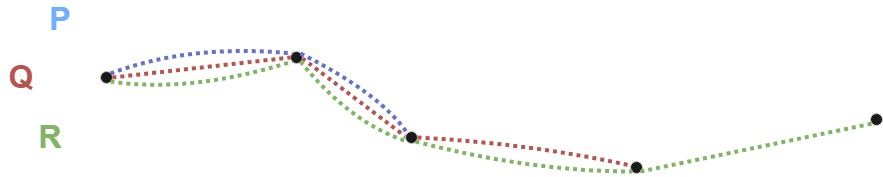
\includegraphics[width=0.9\textwidth]{Related_Works/related_trajes_PQR.jpg}
\caption{\label{fig:related_trajes_PQR}Trajectories $P$, $Q$ and $R$ share 3 points, while trajectories $Q$ and $R$ share 4 points.}
\end{figure}

As the LCSS distance is the sum of all matched points between two trajectories, to be used as a similarity measure it needs to be normalized between 0 and 1. The LCSS similarity score is given by the size of the longest common subsequence ($LCSS(P, Q)$) over the size of the shortest trajectory, i.e., $\dfrac{LCSS(P, Q)}{min(m, n)}$.
Figure \ref{fig:related_trajes_EDR_LCSS} (left) shows the matching of points of trajectories $P$ and $Q$ considering a 15-meter threshold. The LCSS similarity score of $P$ and $Q$ is the {number of points that match} (solid black points) normalized by the size of the shortest trajectory, $LCSS($P$, $Q$) = \dfrac{5}{7} \approx 0.71$.

Chen in \cite{Chen:2005:RFS:1066157.1066213} proposes the Edit Distance on Real sequence (EDR), another similarity measure for raw trajectories. EDR calculates the distance between two trajectories by computing the edit distance between their spatial points. The edit distance between two trajectories is given by summing the distance between their points quantified as 1 if both spatial points do not match, and 0 when they match ({Function} \ref{func:match_EDR}). Using this approach, EDR solves the problem of the gaps in LCSS, by taking into account points that do not match. However, to enforce a match between two points EDR requires that their distance is below a given threshold in all dimensions.

\begin{equation}
%\scriptsize
\label{func:match_EDR}
  match(p, q) = 
  \begin{cases} 
      0 & dist(p, q) \leq \epsilon \\ 
      1 & otherwise\\
  \end{cases}
\end{equation}

A recursive  formalization of EDR is presented in Equation \ref{func:EDR}.

\begin{equation}
%\scriptsize
\label{func:EDR}
  EDR(P, Q) = 
  \begin{cases} 
      0 & \text{if } m = 0\\ 
      0 & \text{if } n = 0\\ 
      min(EDR(<p_2...p_m>,<q_2...q_n>) +  & otherwise\\
      match(p_1, q_1), EDR(<p_2...p_m>, Q) + 1, \\
      EDR(P, <q_2...q_n>) + 1) &
  \end{cases}
\end{equation}

The EDR similarity score is given by the inverse of the number of non-matched points over the size of the longest trajectory, i.e., $1 - \dfrac{EDR(P, Q)}{max(m, n)}$. In the example in Figure \ref{fig:related_trajes_EDR_LCSS} (right), trajectories $P$ and $Q$ only non-match in 2 of their points (solid black) when using a threshold of 15 meters. The EDR similarity score of $P$ and $Q$ is the inverse of the total of non-matched points over the size of the longest trajectory, $EDR($P$, $Q$) = 1 - \dfrac{2}{7} \approx 0.71$.

Comparing the trajectories from Figure \ref{fig:related_trajes_PQR} with EDR, the similarity of $P$ and $Q$ is $EDR(P, Q) = 0.75$ and the similarity of $P$ and $R$ is $EDR(P, R) = 0.60$. These similarity scores show that EDR is robust to {compare trajectories of different sizes}, by giving distinct similarity scores for trajectories of different sizes, solving the drawback of LCSS. Moreover, EDR maintains the robustness to noise of LCSS by using a threshold value in all dimensions.

\begin{figure}[h]
\centering
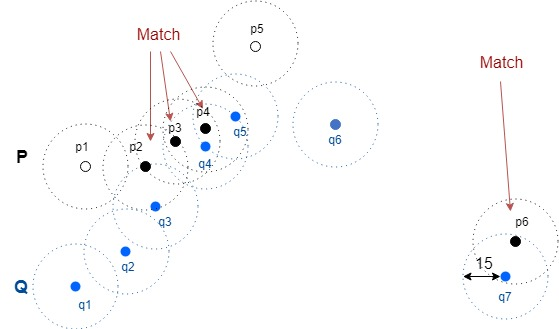
\includegraphics[width=0.45\textwidth]{Related_Works/related_trajes-LCSS.jpg}
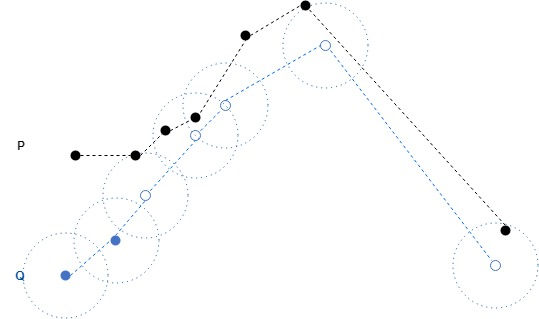
\includegraphics[width=0.45\textwidth]{Related_Works/related_trajes-EDR.jpg}
\caption{\label{fig:related_trajes_EDR_LCSS}(left) LCSS similarity score is the number of matched points normalized by the size of shortest trajectory. (right) EDR distance score is the number of non-matched points normalized by the size of largest trajectory, subtracted by 1.}
\end{figure}

Furtado proposes the \emph{Uncertain Movement Similarity} (UMS) in \cite{Furtado-UMS-2018}. UMS is a parameter-free similarity measure for raw trajectories. UMS was designed exclusively for raw trajectories, using only the spatial dimension. The main contribution of UMS is the elimination of parameters for similarity measuring, by defining a dynamic spatial threshold that is computed automatically according to the distance between the trajectory points. As a consequence, it solves the problem of irregular distribution of trajectory points. UMS represents trajectories as a sequence of movement ellipses, covering the space between two sampled trajectory points.
By using a dynamic ellipse size,  UMS avoids the definition of a radius of fixed size, which is a problem for real applications where the sampling rate can be low and/or irregular, since it is very difficult to estimate such parameter from the user point of view.

Figure \ref{fig:related_trajes_UMS} shows the trajectories $P$ and $Q$ represented as two elliptical trajectories according to UMS. UMS computes the similarity score taking into account three premises: i) \textit{alikeness}: the shapes formed by the union of ellipses look alike; ii) \textit{shareness}: the space covered by both ellipses have a {big shared} area; and iii) \textit{continuity}: the ellipses order represents moving objects traveling continually in the same direction. The limitation in this method lies in it inability to handle trajectories with higher sampling rate, since 

\begin{figure}[!h]
\centering
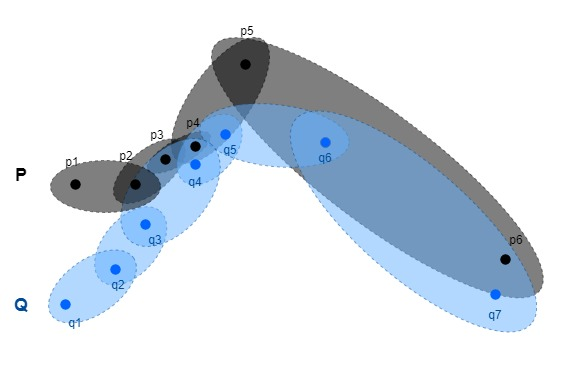
\includegraphics[width=0.75\textwidth]{Related_Works/related_trajes-UMS.jpg}
\caption{\label{fig:related_trajes_UMS}UMS similarity score is given by: i) the shape \textit{alikeness} of ellipses; ii) the \textit{shared} area of ellipses; and iii) the \textit{continuity} of points inside ellipses}
\end{figure}

\subsection{Related works on semantic trajectory similarity measures} \label{sec:related_semantic}

With the definition of semantic trajectory, the creation of new semantic-aware similarity measures are necessary. These new measures may analyze, besides the semantic information, any other information about the trajectory, as for instance the temporal duration of \emph{stops} and \emph{moves}, the spatial point, average speed of the \emph{moves} and so on.

In the following we describe a few semantic trajectory similarity measures, as well as theirs limitations and applications. In order to help understand, we provide some examples, computing similarity scores using trajectories $P$ and $Q$, as previously illustrated in Figure \ref{fig:related_semantic_trajes}. These trajectories are annotated with the spatial coordinates of the \emph{stops} centroids, the time interval of each \emph{stop}, the name and type of the place where a \emph{stop} takes place, the name of the main street where the \emph{move} occurs, as well as the travelled distance and average speed during the \emph{move}.

An early similarity measure considering semantic trajectories is Common Visit Time Interval (CVTI) proposed in \cite{Kang:2009:SMT:1529282.1529580}. It was proposed as a measure for integrating the semantics {and the temporal dimensions of the stops}. It finds the Longest Common Subsequence of two semantic trajectories in {which the semantics is the same and it exists a time intersection between the stops}.
CVTI is strongly based on LCSS, thus presenting the same drawback of LCSS: the inability to penalize gaps of any size in the trajectory, as illustrated in Figure \ref{fig:related_trajes_PQR}. Although CVTI uses different data dimensions, the measure is not extensible for other data dimensions associated with \emph{stops} and \emph{moves}{, since it is handle exclusively the semantic and the time dimensions of \emph{stops}}.

Figure \ref{fig:related_trajes_CVTI} shows the comparison of two trajectories $P$ and $Q$ using the CVTI similarity measure. CVTI finds the Longest Common Subsequence (LCSS) of elements between both trajectories $P$ and $Q$ and gives as similarity score the proportion of time that both trajectories $P$ and $Q$ shared the same \emph{stops}.

\begin{figure}[h]
\centering
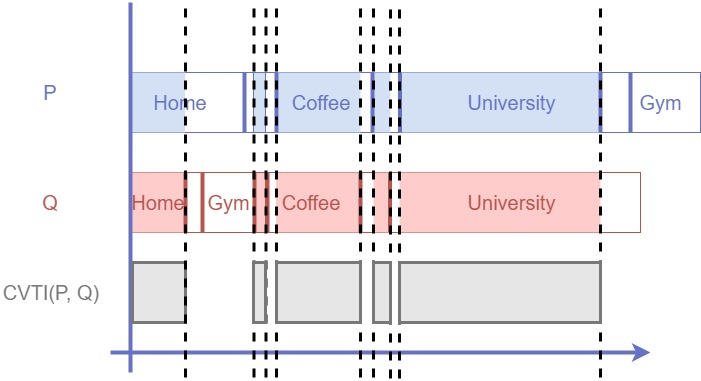
\includegraphics[width=0.65\textwidth]{Related_Works/Semantic_Trajectories_(CVTI).jpg}
\caption{\label{fig:related_trajes_CVTI}CVTI similarity score is the longest common subsequence with time intersection between two trajectories.}
\end{figure}

In \cite{Ying:2010:MUS:1867699.1867703} the measure \emph{Maximal Semantic Trajectory Pattern Similarity} (MSTP) was proposed. It identifies the Longest Common Sequence (LCS) between two semantic trajectories, which are sequences of labels describing the types of places such as $<School, Park, Cinema>$. {MSTP uses only the semantic dimension of trajectories, not being extensible for multiple dimensions, as time and space.} MSTP differentiates from LCSS because it computes a ratio between each trajectory and their common patterns, i.e. the sequence of places visited by both trajectories. The average ratio is used to compute the similarity score, avoiding the drawback of LCSS that does not differentiate matching gaps of different sizes. {The main limitation of the method lies in the exclusively semantic focus, being not extensible to multiple dimensions.}

The work of \cite{Liu:2012:SMM:2442968.2442971} proposed a semantic similarity measure that combines two distances: geographic and semantic. The geographic distance considers three aspects: the distance between the centroids of trajectories, the difference in the length of the trajectories, and the cosine similarity of the directions of subtrajectories. The semantic distance is based on LCSS to find the longest common subsequence of types of places that were visited by the individual. Their approach uses speed variation to split trajectories into subtrajectories, and then the cosine distance is computed between subtrajectories. Limitations of this approach include: i) sensibility to noise in the geographic distance; ii) the time distance is not considered in the distance calculation; and iii) the prevalence of the geographic distance, i.e. two trajectories are similar only if they are similar in space.

\emph{Maximal Travel Match} (MTM)\cite{Xiao:2010:FSU:1869790.1869857} analyzes trajectory similarity in the semantic dimension constrained by time. In order to do that, it proposes a semantic similarity measure that takes into account the semantics of the visited place (e.g., restaurant, university etc.), the sequence of the visited places, the traveled time between places, and the frequency that a place was visited. Two trajectories are more similar if they visited places of the same type, in the same order with similar travel times, according to a time threshold. Limitations of this approach include: i) two semantic trajectories are similar only if they visit the places in the same order; ii) the space dimension is not considered; and iii) MTM measures the similarity considering the whole dataset in order to obtain the frequency of the visited places, what makes the result dependent of the other trajectories in the dataset.

In the work of \cite{Furtado:TGIS12156}, the MSM (Multidimensional Similarity Measuring) measure was proposed, working with multiple dimensions. MSM was designed to handle multidimensional sequences, in which each dimension is independent and each dimension should have its own distance function, i.e., all elements must be homogeneous. MSM is a match-based similarity measure, which means that for each dimension there is a threshold value defining if two elements match or not. Limitations of this approach include: i) the elements homogeneity allows MSM to handle \textit{stops} only, since \textit{stops} and \textit{moves} have distinct attributes, and ii) the order of the elements is not taken into account during the similarity calculation.

{Figure {\ref{fig:related_trajes_MSM}} shows the comparison of two trajectories $P$ and $Q$. In this figure, MSM scores the similarity in a pair-wise fashion, comparing all \emph{stops} from trajectory $P$ with all \emph{stops} of trajectory $Q$. After all stop-to-stop comparisons, MSM computes the similarity score as the sum the best matching score of each \emph{stop}, both $P$ and $Q$ trajectories, over the sum of trajectories length.}

\begin{figure}[h]
\centering
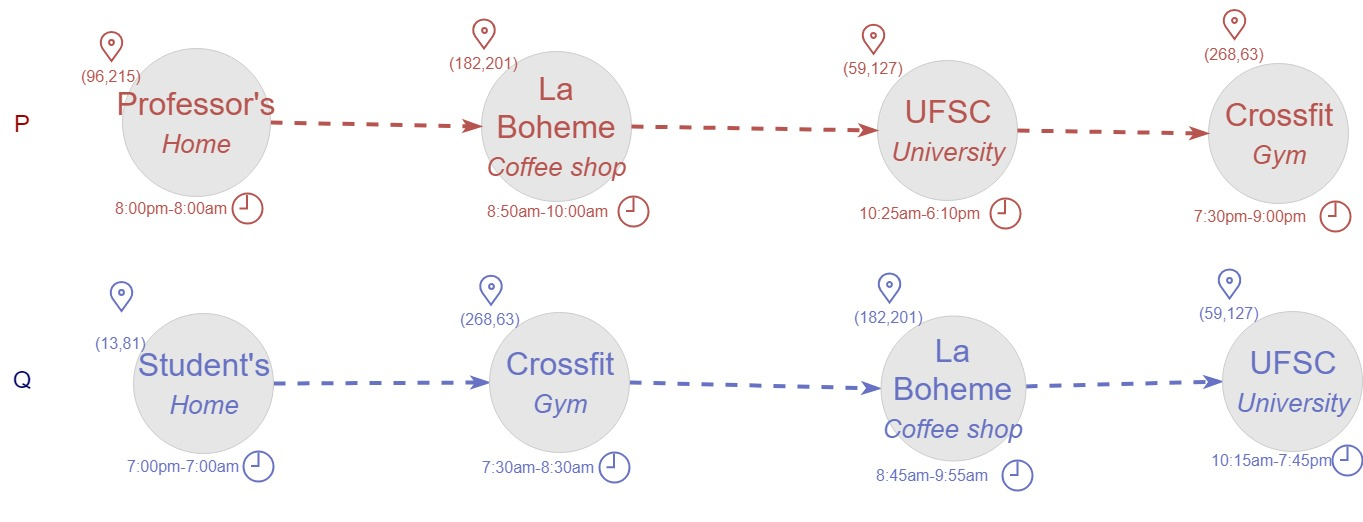
\includegraphics[width=0.65\textwidth]{Related_Works/Semantic_Trajectories_(MSM).jpg}
\caption{\label{fig:related_trajes_MSM}MSM similarity measure computes the similarity score of $P$ and $Q$ using multiple dimensions with partial matching.}
\end{figure}


Cai in \cite{CaiLee2016} proposed a measure that combines the strategies of LCSS \cite{vlachos2002discovering} and MSM\cite{Furtado:TGIS12156} for semantic trajectories. It finds the longest common subsequence between two semantic trajectories. The difference to LCSS is that it does not require the matching in all dimensions, and it does separate the dimensions in two types: compulsory or optional. While all dimensions of the first category should be similar for two elements to match, the optional ones are used only to increase the score, with of their weights being defined in a similar way to MSM.

{Table {\ref{tab:comparative_table}} summarizes the main characteristics of most related measures in comparison to measure proposed in this thesis. We group the measures in two distinct categories: raw or semantic trajectory similarity.

We compare all measures considering: i) if the similarity comparison is performed pairwise by the measure; ii) the time complexity to compute the similarity score; iii) if the measure computes the distance between points in a point matching fashion (i.e., 1 if the distance is greater than a threshold $\epsilon$, 0 otherwise)  or in a continuous fashion (i.e., Euclidean distance, Hausdorff distance, etc); iv) if the measure is robust to noisy data; and v) if the measure is extensible to support multidimensional data.

When comparing the similarity measures for semantic trajectories, we consider: i) if the measure takes into account the \emph{stops} of trajectory; ii) if the measure takes into account the \emph{moves} of trajectory; iii) if the measure allows the use of weights for the dimensions; and iv) if the measures gives a partial score when elements of two trajectories do not match in all dimensions.}

\begin{landscape}
    \begingroup
        \setlength{\tabcolsep}{6pt} % Default value: 6pt
        \renewcommand{\arraystretch}{1.5} % Default value: 1
        \vspace*{\fill}
        \begin{table}[h!]
        \scriptsize
          \centering
          \begin{tabular}{|l|c|c|c|c|c|c|c|c|c|c|c|c|c|}
          	\hline
          	    & \multicolumn{5}{c|}{Raw trajectory similarities} & \multicolumn{7}{c|}{Semantic trajectory similarities}\\
          	\hline
        		& DTWa & wDF & LCSS & EDR & UMS & CVTI & MSTP & Liu & MTM & MSM & Cai & SMSM\\
          	\hline
             Pair-wise similarity & x & x & x & x & x & x &  & x &  & x & x & x \\
          	\hline
             Time-complexity & $n_2$ & $n_2$ & $n_2$ & $n_2$ & $n_2$ & $n_2$ & $n_2$ & $n_2$ & $n_2$ & $n_2$ & $n_2$ & $n_2$\\
          	\hline
             Matching threshold &  &  & x & x &  &  &  & x &  & x & x & x\\
          	\hline
             Robust to noise &  &  & x & x &  & x & x & x & x & x & x & x \\
          	\hline
             Multidimensional & x &  &  &  &  & x &  & x &  & x & x & x\\
          	\hline
             Use stops &  &  &  &  &  & x & x & x & x & x & x &x \\
          	\hline
             Use moves &  &  &  &  &  &  &  &  &  &  &  & x \\
          	\hline
             Dimension weighting &  &  &  &  &  &  &  &  &  & x & x & x \\
          	\hline
             Match elements regardless order &  &  &  &  &  &  &  &  &  & x & x & \\
          	\hline
             Partial matching &  &  &  &  &  &  &  &  &  & x & x & x\\
          	\hline
          \end{tabular}
          \caption{Comparative table}
          \label{tab:comparative_table}
        \end{table}
        \vspace*{\fill}
    \endgroup
\end{landscape}
